\section{\textbf{Outreach Activity}}
Effective science communication, inclusive classrooms, learning environments and outreach activities are vital for the development of science and technology, and upliftment of the society. Our team members have access to several platforms and necessary resources to undertake scientific exposure initiatives which can have an impact on the lives of disadvantaged kids. 
\\

After performing the experiment at CERN, we plan to create an audio-visual demonstration of Art + Physics (an extended version of our BL4S video) to be shared with schools and local educational clubs and societies. We will continue scientific enrichment activities through non-profit organizations such as FLY (Fun Learning Youth) and RAM (Raising a Mathematician Foundation) which strive to bridge the educational gap and spark scientific interest in school students. The focus is free sessions, activities, and the use of hands-on learning as a tool for effective understanding of subjects. Recently, an astronomy seminar and hands-on telescope-making session was held in Nashik, India - 

\begin{center}
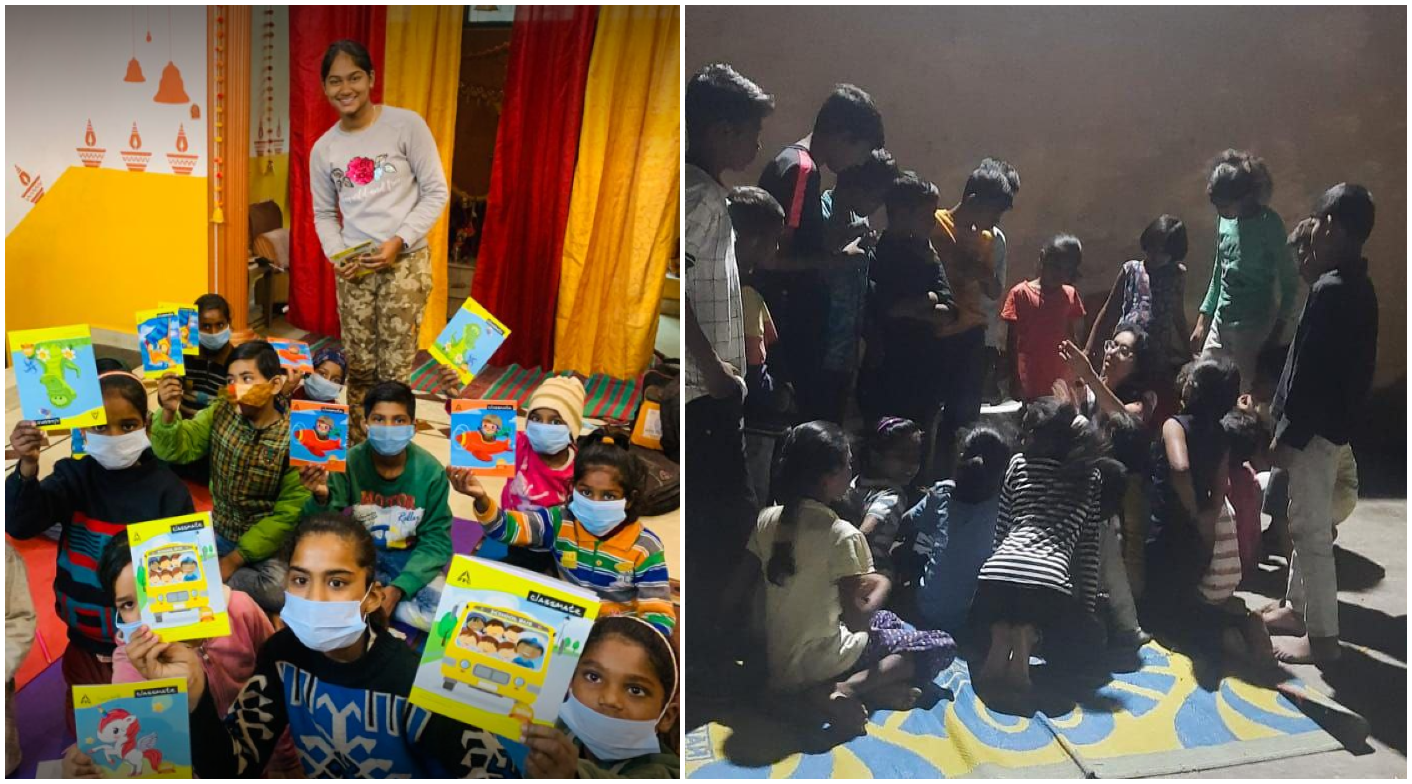
\includegraphics[width=12cm, height=6cm]{Sections/Diagrams/image.png}
\end{center}
\\

Participating in BL4S is an experience which we will cherish for our lifetime. Irrespective of the outcome of the competition, the Pied Pipers pledge to actively contribute towards scientific outreach, envisioning a world where scientific ideas, education and resources are freely accessible to everyone.